\chapter{Aplicação em um sistema real}
\label{chap:holmes}

O objetivo da implementação do algoritmo apresentado no capítulo \ref{chap:implementacao} foi permitir sua implantação no sistema de monitoração de datacenters HOLMES, brevemente descrito neste capítulo. 

A integração com o algoritmo PIP e a arquitetura do software envolvida também são discutidas. Ademais, o resultado final é apresentado e em seguida um caso de uso de sucesso é apresentado.

\section{HOLMES}

O dia a dia da equipe de operação de um datacenter envolve entre outras atividades, o acompanhamento em tempo real de informações provenientes de diferentes máquinas e dispositivos. Centenas de métricas precisam ser monitoradas para garantir que o sistema não apresente quedas de serviço ou \textit{downtime}, o que na maioria dos casos pode provocar perdas significativas de faturamento para o mantenedor do datacenter e seu negócio.

O software HOLMES foi criado com o propósito de fornecer aos operadores de datacenters ferramentas para análise e monitoramento de informações em tempo real, favorecendo o aumento de sua consciência situacional, fator crítico em um ambiente em que muitos equipamentos precisam ser monitorados e a correlação entre eventos para a resolução de um dado problema pode ser difícil, mesmo para operadores experientes.

\section{Integração HOLMES e PIP}
Dentre outras funcionalidades, o software possui uma interface de visualização de gráficos. Nessa interface é possível inspecionar gráficos de métricas coletadas ao longo do tempo provenientes dos itens de configuração cadastrados pelos usuários do sistema.

O termo item de configuração é originário da terminologia ITIL\footnote{ITIL, Information Technology Infrastructure Library.} e pode representar um dispositivo físico como roteador, disco rígido, unidade de processamento, ou qualquer outra métrica lógica como protocolo TCP/IP, HTTP, etc.

Itens de configuração são, em geral, cadastrados no sistema pela equipe de operadores do datacenter. Uma vez cadastrados e configurados, os itens de configuração passam a emitir eventos para um barramento central, de onde são coletados e armazenados. Com base nesses eventos, podemos construir suas séries temporais em sua forma mais bruta. 

Devido a propriedade de alta dimensionalidade, essas séries requerem um processamento adicional antes de serem entregues efetivamente para o usuário final, na interface de visualização. É nesta fase que o algoritmo PIP é empregado, com o papel de reduzir a dimensionalidade dos dados originais e oferecer uma visualização que preserva o comportamento e a forma do gráfico da série original.


\subsection{Arquitetura}
O software de monitoração HOLMES possui um barramento central -- módulo Message broker na figura \ref{fig:overview-architecture} -- destino dos eventos provenientes de diversos equipamentos. Esses dados são coletados e enviados para um módulo de armazenamento denominado \textit{storage}, ilustrado na figura \ref{fig:overview-architecture}.

Na figura \ref{fig:overview-architecture} é demonstrada a arquitetura geral do sistema HOLMES, com destaque para os módulos envolvidos na integração.


\begin{figure}[h!]
  \begin{center}
    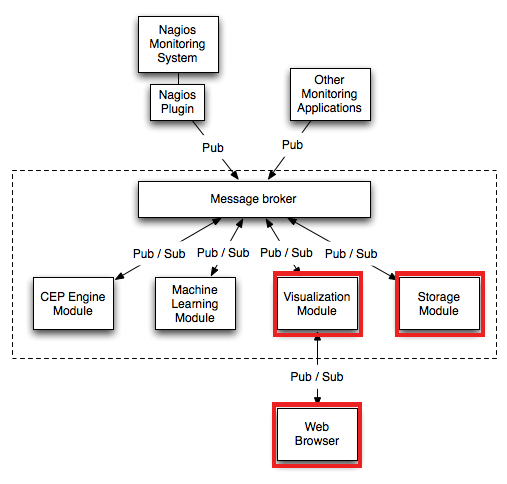
\includegraphics[width=0.6\textwidth]{overview_architecture}
    \centering
    \caption[Arquitetura do sistema HOLMES]{Arquitetura do sistema HOLMES e módulos participantes da integração com o algoritmo PIP}
  \label{fig:overview-architecture}
  \end{center}
\end{figure}

Quando um usuário final requisita uma série temporal através da interface web do sistema HOLMES, o módulo storage é ativado. Os dados originais são coletados e entregues para processamento pelo algoritmo PIP,  devolvidos em seu término\footnote{Os dados são devolvidos em formato JSON (JavaScript Object Notation),  formato de serialização de dados largamente utilizado na Internet.} para o web browser do cliente.

A partir dos pontos perceptivelmente mais importantes no web browser do cliente, seus pontos são entregues finalmente a uma biblioteca Javascript para a plotagem final. Essa estratégia evita que pela rede sejam trafegados todos os pontos originais das séries temporais requisitadas. 

Além disso, ainda que não existissem problemas de banda no tráfego de todos os pontos, outra dificuldade surgiria na etapa de plotagem dos gráficos, no que diz respeito a densidade de pontos. O algoritmo PIP resolve de forma satisfatória essas duas dificuldades.

\subsection{Visualização}
\label{sub:visualizacao}
Para ilustrar o resultado final do que foi exposto até aqui, alguns screenshots foram tirados do sistema HOLMES, que é apenas um codinome para o sistema real: Intelie Event Manager.

As séries temporais que são exibidas para o usuário final estão organizadas na área Histórico do sistema. Na figura \ref{fig:graf-mini}, é possível observar alguns gráficos utilizando o algoritmo PIP. Como o sistema é comercial, alguns nomes foram borrados para manter privacidade de seus clientes. Repare que segundo descrito na seção \ref{sec:limitacoes}, o algoritmo PIP não se comporta muito bem com muitos picos e vales, mas ainda assim apresenta resultados satisfatórios quando o número de PIPs é suficiente, como pode ser observado na figura \ref{fig:tcp-mini}.

\begin{figure}[htb!]
  \begin{center}
    \subfloat[Load mínimo nos últimos 15 minutos]{\label{fig:load-mini}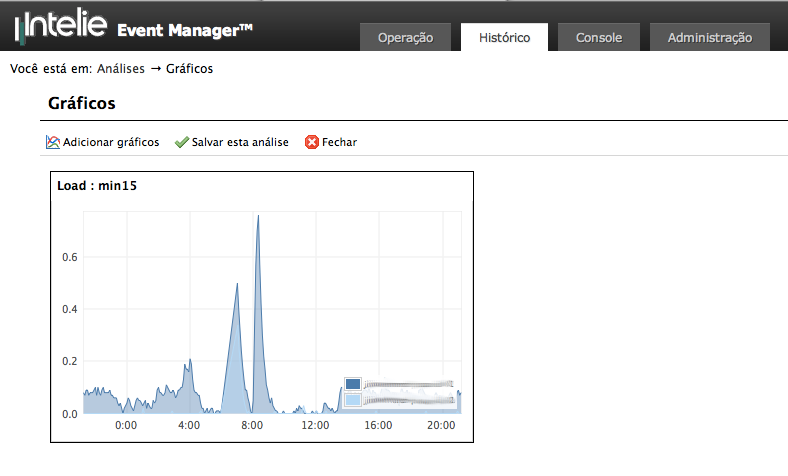
\includegraphics[width=1\textwidth]{load_mini}} \\
    \subfloat[Tempo de resposta do protocolo TCP]{\label{fig:tcp-mini}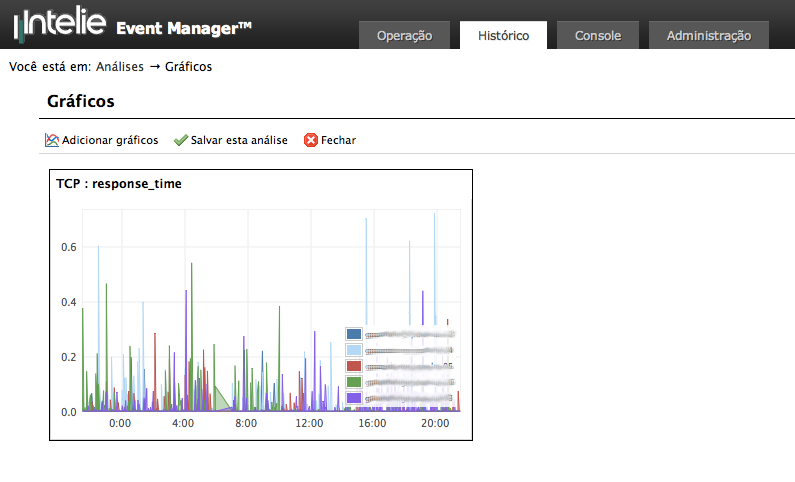
\includegraphics[width=1\textwidth]{tcp_mini}}
    \centering
    \caption{Gráficos gerados a partir do algoritmo PIP no sistema HOLMES}
    \label{fig:graf-mini}
  \end{center}
\end{figure}

\begin{figure}[htb!]
  \begin{center}
    \subfloat[Load mínimo nos últimos 15 minutos]{\label{fig:load-big}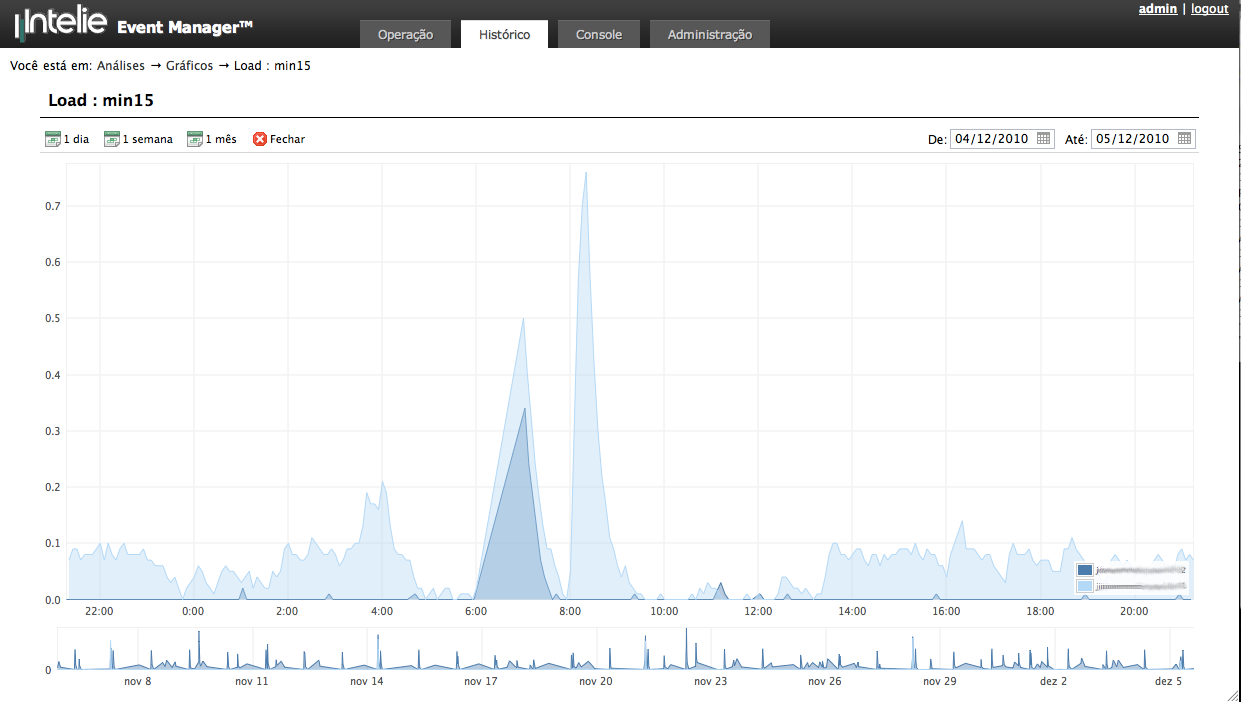
\includegraphics[width=1\textwidth]{load_big}} \\
    \subfloat[Tempo de resposta do protocolo TCP]{\label{fig:tcp-big}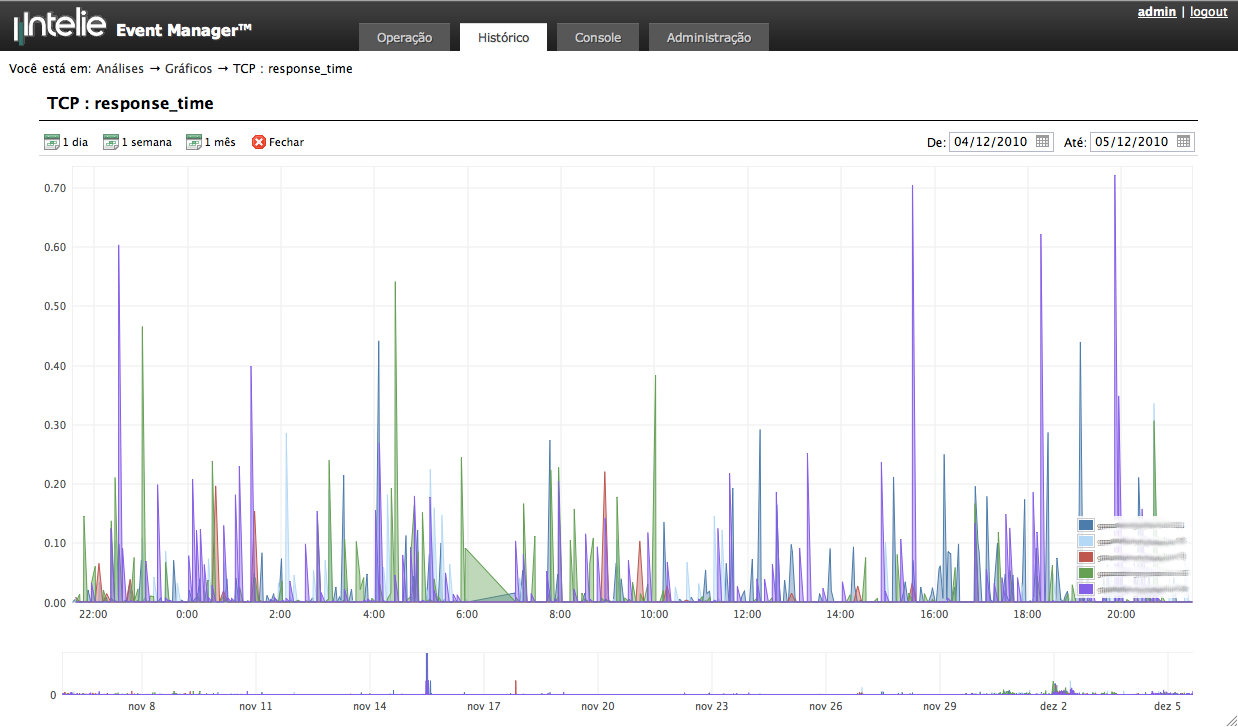
\includegraphics[width=1\textwidth]{tcp_big}}
    \centering
    \caption{Gráficos gerados a partir do algoritmo PIP no sistema HOLMES}
    \label{fig:graf-big}
  \end{center}
\end{figure}

\section{Caso de Uso}
O sistema HOLMES está em uso atualmente em dois grandes datacenters do Brasil: Globo.com e iG.

Versões anteriores do sistema HOLMES contavam com técnicas de média sobre média, brevemente discutidas na seção \ref{sec:time-series-datacenter}, que desfiguravam a forma geral do gráfico, confundindo usuários finais em sua interpretação dos dados.

Operadores destes datacenters manifestaram diminuição no tempo de detecção de falhas de problemas em equipamentos de seus servidores após a implementação da interface de visualização utilizando o algoritmo PIP.
